%% Phase-4 migration of v1.1 Part II, Chapter 1 (source lines 1649--2186).
%% Body statements only.  The eight complete proofs are in
%% annex/p02/propositional-syntax-semantics.tex.  Post1941 is intentionally
%% cited here; the P2 finalizer supplies that verified bibliography entry.
%% Shared finalizer dependency: register \upsilon in the P02 symbol intake as the
%% local uniform-substitution map (the usual alternatives are already reserved
%% for sentence metavariables and label-renaming maps in the P2.1 scope).

\chapter{Propositional Syntax and Semantics}
\label{sec:p02-propositional-syntax-semantics}

Classical propositional logic combines an inductively generated language with
two-valued semantics.  The presentation preserves the verified source account
\cite{EbbinghausFlumThomas1994,OpenLogic2026}, while the Part~1 registry fixes
the handbook-wide symbols and binding conventions.

\section{Alphabet, grammar, and readability}
\label{sec:p02-propositional-grammar}

\begin{hbdefinition}{def:p02-propositional-alphabet}{Alphabet, propositional@Propositional alphabet}
The \emph{propositional alphabet}\index{propositional variable} consists of
the variables \(\mathsf{Prop}\defeq\{p_n:n\in\N\}\), the nullary connective
\(\bottom\), the unary connective \(\neg\), the binary connectives
\(\land,\lor,\to\), and the punctuation symbols \((\) and \()\).  All these
symbols are distinct.  Variables are object-language symbols;
\(\varphi,\psi,\chi\) are metalinguistic formula variables, while
\(P,Q,R,S\) denote specified members of \(\mathsf{Prop}\).
\end{hbdefinition}

\begin{hbdefinition}{def:p02-propositional-formula}{Formula, propositional@Propositional formula}
The set \(\mathsf{Fm}_{\mathsf{CPL}}\) of \emph{propositional formulas} is
the least set of strings such that: \(p_n\) belongs to it for every
\(n\in\N\); \(\bottom\) belongs to it; if \(\varphi\) belongs to it, then
\(\neg\varphi\) belongs to it; and if \(\varphi,\psi\) belong to it and
\(\circ\in\{\land,\lor,\to\}\), then
\((\varphi\circ\psi)\) belongs to it.  No other string is a formula.  Thus
\[
 \varphi ::= p_n\mid\bottom\mid\neg\varphi
 \mid(\varphi\land\psi)\mid(\varphi\lor\psi)
 \mid(\varphi\to\psi).
\]
\end{hbdefinition}

\begin{hbconvention}{def:p02-parenthesis-convention}{Parenthesis omission and binding}
The grammar's parentheses are object-language symbols.  Expository displays
may omit outermost parentheses under the following convention:
\(\neg\) binds most tightly; \(\land\) and \(\lor\) are left associative;
\(\to\) is right associative; and the four levels occur in that order of
decreasing binding strength.  These are typographical abbreviations, not
formation clauses.
\end{hbconvention}

\begin{hbdefinition}{def:p02-defined-connectives}{Connective, defined@Defined connectives}
The signs \(\topv\) and \(\leftrightarrow\) are metalinguistic
abbreviations, not new constructors:
\[
 \topv\defeq\neg\bottom,
 \qquad
 (\varphi\leftrightarrow\psi)
 \defeq((\varphi\to\psi)\land(\psi\to\varphi)).
\]
\index{truth constant!true}\index{biconditional}
\end{hbdefinition}

\begin{hbdefinition}{def:p02-finite-connectives}{Conjunction, finite@Finite conjunction and disjunction}
For an ordered finite sequence \(\varphi_1,\ldots,\varphi_n\) with
\(n>0\), put \(C_n=\varphi_n\), \(D_n=\varphi_n\), and, downward,
\(C_i=(\varphi_i\land C_{i+1})\) and
\(D_i=(\varphi_i\lor D_{i+1})\).  Define
\(\bigwedge_{i=1}^{n}\varphi_i\defeq C_1\) and
\(\bigvee_{i=1}^{n}\varphi_i\defeq D_1\).  For \(n=0\), these are
\(\topv\) and \(\bottom\), respectively.  An indexed display is used only
after its index order is fixed.  This metalinguistic convention assigns one
formula string to every such display and is intentionally right associated,
independently of the convention for unparenthesized binary chains.
\index{disjunction!finite}
\end{hbdefinition}

\begin{hblemma}{thm:p02-parenthesis-counting}{proved=annex:p2.1.1}{Parenthesis counting}
Every formula contains equally many left and right parentheses.  Moreover,
at every binary-connective occurrence, the number of left parentheses
strictly preceding it exceeds the number of right parentheses strictly
preceding it.
\end{hblemma}

\begin{hbtheorem}{thm:p02-unique-readability}{proved=annex:p2.1.2}{Unique readability}
Every formula satisfies exactly one formation clause.  In a negation its
immediate subformula is unique; in a binary formula its main connective and
its two immediate subformulas are unique.
\end{hbtheorem}

\begin{hbdefinition}{def:p02-complexity-subformula}{Complexity and subformula}
Formula \emph{complexity}\index{formula complexity} is given by
\[
 c(p_n)=c(\bottom)=0,\qquad
 c(\neg\varphi)=c(\varphi)+1,\qquad
 c(\varphi\circ\psi)=c(\varphi)+c(\psi)+1.
\]
The \emph{subformula set}\index{subformula} is given recursively by
\[
\begin{aligned}
 \operatorname{Sub}(p_n)&=\{p_n\},&
 \operatorname{Sub}(\bottom)&=\{\bottom\},\\
 \operatorname{Sub}(\neg\varphi)&=\{\neg\varphi\}\cup
   \operatorname{Sub}(\varphi),\\
 \operatorname{Sub}(\varphi\circ\psi)&=\{\varphi\circ\psi\}\cup
   \operatorname{Sub}(\varphi)\cup\operatorname{Sub}(\psi),
\end{aligned}
\]
where \(\circ\in\{\land,\lor,\to\}\).
\end{hbdefinition}

\begin{figure}[tp]
\centering
\begin{tikzpicture}[level distance=9mm,
 every node/.style={inner sep=1.5pt},
 level 1/.style={sibling distance=36mm},
 level 2/.style={sibling distance=18mm},
 level 3/.style={sibling distance=10mm}]
\node {\(\to\)}
 child {node {\(\land\)}
   child {node {\(\neg\)} child {node {\(P\)}}}
   child {node {\(Q\)}}}
 child {node {\(\lor\)}
   child {node {\(R\)}}
   child {node {\(S\)}}};
\end{tikzpicture}
\caption{The syntax tree of
\(((\neg P\land Q)\to(R\lor S))\).  Internal nodes are connective
occurrences, subtrees are subformula occurrences, and
Theorem~\ref{thm:p02-unique-readability} makes the parse unique
(apparatus A-114).}
\label{fig:p02-formula-syntax-tree}
\end{figure}

\section{Valuations and semantic congruence}
\label{sec:p02-propositional-semantics}

\begin{hbdefinition}{def:p02-valuation}{Valuation, propositional@Propositional valuation}
Let \(\mathbb B\defeq\{0,1\}\).  A \emph{valuation} is a
function \(v:\mathsf{Prop}\to\mathbb B\).  Its unique recursive extension
\(\widehat v:\mathsf{Fm}_{\mathsf{CPL}}\to\mathbb B\) satisfies
\[
\begin{array}{rcl}
\widehat v(p_n)&=&v(p_n),\\
\widehat v(\bottom)&=&0,\\
\widehat v(\neg\varphi)=1&\text{iff}&\widehat v(\varphi)=0,\\
\widehat v(\varphi\land\psi)=1&\text{iff}&
 \widehat v(\varphi)=1\text{ and }\widehat v(\psi)=1,\\
\widehat v(\varphi\lor\psi)=1&\text{iff}&
 \widehat v(\varphi)=1\text{ or }\widehat v(\psi)=1,\\
\widehat v(\varphi\to\psi)=0&\text{iff}&
 \widehat v(\varphi)=1\text{ and }\widehat v(\psi)=0.
\end{array}
\]
Write \(v\entails\varphi\) iff \(\widehat v(\varphi)=1\).
\index{truth value}
\end{hbdefinition}

\begin{hblemma}{thm:p02-propositional-coincidence}{proved=annex:p2.1.3}{Coincidence for propositional formulas}
If valuations \(v,w\) agree on every variable occurring in \(\varphi\),
then \(\widehat v(\varphi)=\widehat w(\varphi)\).
\end{hblemma}

\begin{hbdefinition}{def:p02-propositional-semantic-notions}{Semantics, propositional@Propositional semantic notions}
Let \(\Gamma\subseteq\mathsf{Fm}_{\mathsf{CPL}}\) and
\(\varphi,\psi\in\mathsf{Fm}_{\mathsf{CPL}}\).  A valuation \emph{satisfies}
\(\Gamma\), written \(v\entails\Gamma\), iff it satisfies every member.
The set is \emph{satisfiable} iff some valuation satisfies it.  The formula
\(\varphi\) is \emph{valid}, written \(\entails\varphi\), iff every valuation
satisfies it.  It is a \emph{semantic consequence} of \(\Gamma\), written
\(\Gamma\entails\varphi\), iff every valuation satisfying \(\Gamma\) also
satisfies \(\varphi\).  Finally,
\(\varphi\Leftrightarrow\psi\) means that every valuation gives the two
formulas the same truth value; this is \emph{logical equivalence}.
\index{satisfaction!propositional}\index{satisfiability!propositional}
\index{validity!propositional}\index{semantic consequence!propositional}
\index{logical equivalence!propositional}
\end{hbdefinition}

Thus \(\varnothing\entails\varphi\) iff \(\entails\varphi\).  A
countervaluation to \(\Gamma\entails\varphi\) satisfies \(\Gamma\) and
falsifies \(\varphi\).  Formula equivalence is always written
\(\Leftrightarrow\).

\begin{hbdefinition}{def:p02-uniform-substitution}{Substitution, uniform@Uniform substitution}
A \emph{uniform substitution}\index{formula instance} is a function
\(\upsilon:\mathsf{Prop}\to\mathsf{Fm}_{\mathsf{CPL}}\).  Its instance map is
defined recursively by
\[
 p_n[\upsilon]=\upsilon(p_n),\quad \bottom[\upsilon]=\bottom,\quad
 (\neg\varphi)[\upsilon]=\neg(\varphi[\upsilon]),\quad
 (\varphi\circ\psi)[\upsilon]=
   (\varphi[\upsilon]\circ\psi[\upsilon]).
\]
\end{hbdefinition}

\begin{hbtheorem}{thm:p02-uniform-substitution}{cited=Kleene1952}{Uniform-substitution theorem}
For every uniform substitution \(\upsilon\): if \(\entails\varphi\), then
\(\entails\varphi[\upsilon]\); and if
\(\varphi\Leftrightarrow\psi\), then
\(\varphi[\upsilon]\Leftrightarrow\psi[\upsilon]\).
\end{hbtheorem}

\begin{hbtheorem}{thm:p02-replacement}{cited=Kleene1952}{Replacement theorem}
Logical equivalence is an equivalence relation and a congruence for each
primitive connective.  Hence, if \(\psi\Leftrightarrow\chi\) and
\(\varphi'\) results from \(\varphi\) by replacing any chosen occurrences
of the subformula \(\psi\) by \(\chi\), then
\(\varphi\Leftrightarrow\varphi'\).
\end{hbtheorem}

The preceding two statements fill depth row D-P2-010.  They distinguish
uniform substitution for variables from replacement at selected subformula
occurrences.

\begin{hbtheorem}{thm:p02-equivalence-laws}{cited=Kleene1952}{Standard equivalence laws}
Every row of Table~\ref{tab:p02-equivalence-laws} is a logical equivalence
schema under every substitution of formulas for its metavariables.
\end{hbtheorem}

\begingroup\small
\begin{longtable}{@{}clp{0.62\textwidth}@{}}
\caption{Standard propositional equivalence laws (apparatus A-027).}
\label{tab:p02-equivalence-laws}\\
\toprule Row & Name & Citable equivalence schema \\
\midrule\endfirsthead
\toprule Row & Name & Citable equivalence schema \\
\midrule\endhead
E1 & Idempotence & \(\varphi\land\varphi\Leftrightarrow\varphi\),
 \(\varphi\lor\varphi\Leftrightarrow\varphi\) \\
E2 & Commutativity & \(\varphi\land\psi\Leftrightarrow\psi\land\varphi\),
 \(\varphi\lor\psi\Leftrightarrow\psi\lor\varphi\) \\
E3 & Associativity & \((\varphi\land\psi)\land\chi\Leftrightarrow
 \varphi\land(\psi\land\chi)\), and its \(\lor\)-dual \\
E4 & Absorption & \(\varphi\land(\varphi\lor\psi)\Leftrightarrow\varphi\),
 \(\varphi\lor(\varphi\land\psi)\Leftrightarrow\varphi\) \\
E5 & Distribution & \(\varphi\land(\psi\lor\chi)\Leftrightarrow
 (\varphi\land\psi)\lor(\varphi\land\chi)\) \\
E6 & Distribution & \(\varphi\lor(\psi\land\chi)\Leftrightarrow
 (\varphi\lor\psi)\land(\varphi\lor\chi)\) \\
E7 & De Morgan & \(\neg(\varphi\land\psi)\Leftrightarrow
 \neg\varphi\lor\neg\psi\) \\
E8 & De Morgan & \(\neg(\varphi\lor\psi)\Leftrightarrow
 \neg\varphi\land\neg\psi\) \\
E9 & Double negation & \(\neg\neg\varphi\Leftrightarrow\varphi\) \\
E10 & Material implication & \(\varphi\to\psi\Leftrightarrow
 \neg\varphi\lor\psi\) \\
E11 & Contraposition & \(\varphi\to\psi\Leftrightarrow
 \neg\psi\to\neg\varphi\) \\
E12 & Exportation & \((\varphi\land\psi)\to\chi\Leftrightarrow
 \varphi\to(\psi\to\chi)\) \\
E13 & Negated implication & \(\neg(\varphi\to\psi)\Leftrightarrow
 \varphi\land\neg\psi\) \\
E14 & Units & \(\varphi\land\topv\Leftrightarrow\varphi\),
 \(\varphi\lor\bottom\Leftrightarrow\varphi\) \\
E15 & Annihilation & \(\varphi\land\bottom\Leftrightarrow\bottom\),
 \(\varphi\lor\topv\Leftrightarrow\topv\) \\
E16 & Complementation & \(\varphi\land\neg\varphi\Leftrightarrow\bottom\),
 \(\varphi\lor\neg\varphi\Leftrightarrow\topv\) \\
E17 & Unit negation & \(\neg\topv\Leftrightarrow\bottom\),
 \(\neg\bottom\Leftrightarrow\topv\) \\
E18 & Biconditional & \(\varphi\leftrightarrow\psi\Leftrightarrow
 (\varphi\to\psi)\land(\psi\to\varphi)\) \\
E19 & Biconditional cases & \(\varphi\leftrightarrow\psi\Leftrightarrow
 (\varphi\land\psi)\lor(\neg\varphi\land\neg\psi)\) \\
\bottomrule
\end{longtable}
\endgroup

\section{Translation from controlled prose}
\label{sec:p02-controlled-prose}

A translation includes a key assigning a variable to every atomic statement;
without that key, a formula does not preserve the prose content
\cite{OpenLogic2026}.  Truth-functional translation does not encode emphasis,
causal force, or conversational contrast.

\begin{hbexample}{def:p02-unless-example}{Unless with a compound key}
Let \(P\) mean ``the archive is readable'' and \(Q\) mean ``the checksum is
valid.''  ``The archive is readable unless the checksum is invalid'' has the
form \(P\) unless \(\neg Q\), hence translates first as
\(\neg\neg Q\to P\).  Replacing this by \(Q\to P\) is a separate
equivalence-law step, not part of the initial translation.
\end{hbexample}

\begingroup\small
\begin{longtable}{@{}p{0.31\textwidth}p{0.27\textwidth}p{0.34\textwidth}@{}}
\caption{Controlled-English translation guide (apparatus A-032).}
\label{tab:p02-controlled-english}\\
\toprule Prose form & Formula & Scope note \\
\midrule\endfirsthead
\toprule Prose form & Formula & Scope note \\
\midrule\endhead
if \(P\), then \(Q\) & \(P\to Q\) & ``if'' supplies the antecedent \\
\(P\) only if \(Q\) & \(P\to Q\) & ``only if'' supplies the consequent \\
\(P\) if \(Q\) & \(Q\to P\) & the following condition is sufficient \\
\(P\) iff \(Q\) & \(P\leftrightarrow Q\) & both conditionals \\
\(P\) unless \(Q\) & \(\neg Q\to P\) & inclusive unless; equivalent to \(P\lor Q\) \\
neither \(P\) nor \(Q\) & \(\neg P\land\neg Q\) & not \(\neg P\lor\neg Q\) \\
not both \(P\) and \(Q\) & \(\neg(P\land Q)\) & weaker than neither \\
\(P\) or \(Q\), inclusively & \(P\lor Q\) & true when both hold \\
exactly one of \(P,Q\) & \((P\lor Q)\land\neg(P\land Q)\) & exclusive disjunction \\
\(P\), but \(Q\) & \(P\land Q\) & contrast has no truth-functional effect \\
\(P\) is necessary for \(Q\) & \(Q\to P\) & the necessary condition follows \\
\(P\) is sufficient for \(Q\) & \(P\to Q\) & the sufficient condition precedes \\
\bottomrule
\end{longtable}
\endgroup

\section{Clauses and normal forms}
\label{sec:p02-propositional-normal-forms}

\begin{hbdefinition}{def:p02-propositional-clause}{Clause, propositional@Propositional literals and clauses}
A \emph{literal}\index{literal!propositional} is \(p_n\) or \(\neg p_n\).
A \emph{clause}\index{clause!propositional} is a finite set of literals, so
order and repetition are absent.  Resolution requires the complement to
remain a literal even when its input is already negated.  Accordingly, within
the propositional-clause scope, define the metalinguistic involution
\[
 \overline{p_n}\defeq\neg p_n,
 \qquad
 \overline{\neg p_n}\defeq p_n.
\]
It differs from merely prefixing object-language \(\neg\) in the second case,
and is used by the resolution entry.  A clause \(C\) is
\emph{tautological} iff \(L,\overline L\in C\) for some literal \(L\); its
formula interpretation is then valid.
\index{literal!complement}\index{clause!tautological}

Put
\(\operatorname{code}(p_n)=2n\) and
\(\operatorname{code}(\neg p_n)=2n+1\).  If a nonempty clause \(C\) has,
in increasing code order, the members \(L_1,\ldots,L_k\), define
\(D_k=L_k\) and \(D_i=(L_i\lor D_{i+1})\) downward, and set
\[
 \operatorname{form}_{\mathsf{CPL}}(C)\defeq
 \begin{cases}\bottom,&C=\varnothing,\\D_1,&C\ne\varnothing.\end{cases}
\]
This is a metalinguistic function from clauses to formula strings, not a
formula constructor.  A valuation satisfies \(C\) iff it satisfies
\(\operatorname{form}_{\mathsf{CPL}}(C)\).  For an arbitrary set \(S\) of
clauses, define
\[
 v\entails S \quad\text{iff}\quad
 (\forall C\in S)\,v\entails C;
\]
thus clause-set satisfaction is conjunctive, and \(S\) is satisfiable iff
some valuation satisfies it.  If \(C\in S\) is tautological, then
\(v\entails S\) iff \(v\entails S\setminus\{C\}\) for every valuation \(v\).
Consequently, deleting any tautological members preserves exactly the
satisfying valuations of \(S\).
\index{formula interpretation!clause}
\index{clause set!satisfaction}\index{satisfiability!clause set}
\end{hbdefinition}

\begin{hbdefinition}{def:p02-propositional-normal-forms}{Normal form!propositional}
A formula is in \emph{negation normal form} (NNF) iff it is built from
literals and \(\bottom,\topv\) using only \(\land,\lor\).  It is in
\emph{conjunctive normal form} (CNF) iff it is \(\topv\), or it is the
right-associated finite conjunction of the formula interpretations of a
nonempty ordered list of clauses.  It is in \emph{disjunctive normal form}
(DNF) iff it is a finite disjunction of finite conjunctions of literals.
The empty conjunction is \(\topv\); the empty disjunction is \(\bottom\).
\index{negation normal form}\index{conjunctive normal form}
\index{disjunctive normal form}
\end{hbdefinition}

\begin{hblemma}{thm:p02-clause-satisfaction}{proved=annex:p2.1.4}{Satisfaction of clauses and clause conjunctions}
Let \(v\) be a valuation.  For every clause \(C\),
\(v\entails\operatorname{form}_{\mathsf{CPL}}(C)\) iff
\(v\entails L\) for some \(L\in C\).  For \(m>0\), \(v\) satisfies the
right-associated conjunction of
\(\operatorname{form}_{\mathsf{CPL}}(C_1),\ldots,
\operatorname{form}_{\mathsf{CPL}}(C_m)\) iff it satisfies every conjunct.
\end{hblemma}

\begin{hbtheorem}{thm:p02-negation-normal-form}{proved=annex:p2.1.5}{Negation normal form}
Every propositional formula is logically equivalent to a formula in NNF.
\end{hbtheorem}

\begin{hbtheorem}{thm:p02-conjunctive-disjunctive-normal-form}{proved=annex:p2.1.6}{Conjunctive and disjunctive normal forms}
Every propositional formula is logically equivalent both to a DNF formula and
to a CNF formula.
\end{hbtheorem}

Equivalent normal forms may be exponentially larger than their input.  When
only satisfiability is to be preserved, use the following Part~12 forward
link rather than silently claiming equivalence.

\begin{hbdefinition}{def:p02-equisatisfiability}{Equisatisfiability}
Two formulas, possibly over different variable sets, are
\emph{equisatisfiable} iff either both are satisfiable or both are
unsatisfiable.  This is a metalinguistic relation between formulas and is
strictly weaker than logical equivalence when fresh variables are introduced.
\end{hbdefinition}

\begin{hbtheorem}{thm:p02-tseitin}{cited=Prestwich2021}{Tseitin transformation}
For every formula \(\varphi\), a linear-time transformation produces a CNF
formula \(T_\varphi\) of linear size over the original variables and fresh
auxiliary variables such that, for every valuation \(v\) of the original
variables,
\[
 v\entails\varphi
 \quad\text{iff}\quad
 \text{there is a unique extension }w\supseteq v
 \text{ with }w\entails T_\varphi.
\]
The uniqueness is for the full biconditional definitional constraints.  Thus
\(T_\varphi\) is equisatisfiable with \(\varphi\), but is not a
same-vocabulary logically equivalent formula.  The historical construction is
due to Tseitin~\cite{Tseitin1968}; the Part~12 automation entry gives the gate
constraints and worked construction.  This is depth row D-P2-007.
\end{hbtheorem}

\section{Duality}
\label{sec:p02-propositional-duality}

\begin{hbdefinition}{def:p02-nnf-dual}{Duality, propositional@Propositional duality}
To make the unit swap literal rather than dependent on expanding
\(\topv\defeq\neg\bottom\), use the metalinguistic NNF presentation
\[
 \alpha ::= L\mid\bottom\mid\topv\mid(\alpha\land\beta)
             \mid(\alpha\lor\beta),
\]
where \(L\) is a literal.  This presentation is necessary only to retain the
two displayed units as distinct abbreviation forms; it adds no object-language
constructor and differs from ordinary NNF in no semantic value.  Its
\emph{dual} is the metalinguistic operation
\[
\begin{aligned}
 L^{\mathrm d}&=L,&
 \bottom^{\mathrm d}&=\topv,&
 \topv^{\mathrm d}&=\bottom,\\
 (\alpha\land\beta)^{\mathrm d}
   &=\alpha^{\mathrm d}\lor\beta^{\mathrm d},&&
 (\alpha\lor\beta)^{\mathrm d}
   =\alpha^{\mathrm d}\land\beta^{\mathrm d}.
\end{aligned}
\]
Thus the presentation device and the dual operation have metalinguistic
standing, are nonredundant exactly at the unit leaves, and are used below to
state the CNF--DNF correspondence without syntactic ambiguity.
\index{dual formula}\index{duality!propositional}
\end{hbdefinition}

\begin{hbtheorem}{thm:p02-propositional-duality}{proved=annex:p2.1.8}{Duality theorem}
Let \(\bar v(p)=1-v(p)\).  For every NNF
presentation \(\alpha\),
\[
 v\entails\alpha^{\mathrm d}\quad\text{iff}\quad
 \bar v\not\entails\alpha.
\]
Consequently dualization is an involution, preserves logical equivalence,
exchanges valid formulas with unsatisfiable formulas, and exchanges CNF with
DNF.  This fills depth row D-P2-003.
\end{hbtheorem}

\begingroup\small
\begin{longtable}{@{}lll@{}}
\caption{The NNF duality dictionary (apparatus A-028).}
\label{tab:p02-duality}\\
\toprule Object & Dual & Consequence \\
\midrule\endfirsthead
\toprule Object & Dual & Consequence \\
\midrule\endhead
literal \(L\) & \(L\) & complemented valuation reverses its value \\
\(\bottom\) & \(\topv\) & false and true units swap \\
\(\land\) & \(\lor\) & outer conjunction becomes disjunction \\
\(\lor\) & \(\land\) & outer disjunction becomes conjunction \\
CNF & DNF & clauses become conjunctions of literals \\
valid & unsatisfiable & Theorem~\ref{thm:p02-propositional-duality} \\
\bottomrule
\end{longtable}
\endgroup

\section{Truth functions and Post's criterion}
\label{sec:p02-functional-completeness}

\begin{hbdefinition}{def:p02-completeness-scopes}{Functional completeness}
An \(n\)-ary \emph{truth function}\index{truth function} is a function
\(\mathbb B^n\to\mathbb B\).  A connective signature supplies one such
function for each of its connectives, and its formulas are generated using
those arities.  Such a formula \(\varphi\) \emph{represents}
\(f:\mathbb B^n\to\mathbb B\) in variables \(p_1,\ldots,p_n\) iff its
variables are among those displayed and, whenever \(v(p_i)=a_i\),
\(\widehat v(\varphi)=f(a_1,\ldots,a_n)\); coincidence makes this
well-defined.  A \emph{clone}\index{clone!truth functions} is a family of
positive-arity truth functions containing every projection and closed under
composition (superposition).

Two completeness scopes are required: a signature is
\emph{positive-arity functionally complete} iff it represents every
\(f:\mathbb B^n\to\mathbb B\) for every \(n\geq1\); it is
\emph{nullary-inclusive functionally complete} iff the same holds for every
\(n\geq0\), with a closed formula required when \(n=0\).  These are
metalinguistic properties of connective signatures.  The distinction is
necessary because a signature containing only NAND or only NOR has no closed
formula; it is nonredundant only at arity zero.  The source basis theorem uses
the nullary-inclusive notion, whereas Post's clone criterion and the standard
single-connective claim use the positive-arity notion.
\index{functional completeness!positive arity}
\index{functional completeness!nullary inclusive}
\end{hbdefinition}

\begin{hbtheorem}{thm:p02-functional-basis}{proved=annex:p2.1.7}{A functionally complete basis}
Primitive \(\neg\), \(\land\), and nullary \(\bottom\) form a
nullary-inclusive functionally complete signature.
\end{hbtheorem}

The following modern membership tests are calibrated by
\cite{PelletierMartin1990}, while the classification itself is Post's.

\begin{hbtheorem}{thm:p02-post-criterion}{cited=Post1941}{Post's functional-completeness criterion}
Let \(C\) be a set of positive-arity truth functions, and let
\(\langle C\rangle\) denote the intersection of all clones containing
\(C\), the clone it generates.  Then
\(\langle C\rangle\) is the clone of all positive-arity Boolean operations
iff, for each of
\(\mathsf T_0,\mathsf T_1,\mathsf M,\mathsf L,\mathsf S\) in
Table~\ref{tab:p02-post-maximal-clones}, some member of \(C\) lies outside
that class.  These five classes are exactly the maximal proper clones; every
proper clone is contained in at least one of them.
\end{hbtheorem}

The criterion makes negative results one-line containment arguments.  After
replacing a displayed nullary constant by its unary constant operation,
\(\{\land,\lor,\bottom,\topv\}\) generates a clone contained in
\(\mathsf M\), so it cannot define negation;
\(\{\neg,\leftrightarrow\}\) generates one contained in \(\mathsf L\), so
it cannot define conjunction; and the clone generated by \(\{\to\}\) is
contained in \(\mathsf T_1\), so implication alone is incomplete.

\begingroup\scriptsize
\begin{longtable}{@{}lp{0.34\textwidth}p{0.22\textwidth}p{0.22\textwidth}@{}}
\caption{The five maximal clones and their membership tests (apparatus A-029).
The displayed constant functions have positive arity and ignore every input;
they are not nullary connective symbols.}
\label{tab:p02-post-maximal-clones}\\
\toprule Clone & Exact membership test for \(f:\mathbb B^n\to\mathbb B\), \(n\geq1\)
 & Sample members & Sample nonmembers \\
\midrule\endfirsthead
\toprule Clone & Exact membership test for \(f:\mathbb B^n\to\mathbb B\), \(n\geq1\)
 & Sample members & Sample nonmembers \\
\midrule\endhead
\(\mathsf T_0\) & \(f(0,\ldots,0)=0\)
 & \(\land,\lor\), exclusive-or, constant 0 & \(\neg,\to\), NAND, NOR \\
\(\mathsf T_1\) & \(f(1,\ldots,1)=1\)
 & \(\land,\lor,\to\), constant 1 & \(\neg\), exclusive-or, NAND, NOR \\
\(\mathsf M\) & monotone for the pointwise order \(0<1\)
 & \(\land,\lor\), both constant functions & \(\neg,\to\), exclusive-or, NAND, NOR \\
\(\mathsf L\) & affine over \(\mathbb F_2\):
 \(f(a)=c_0+c_1a_1+\cdots+c_na_n\)
 & \(\neg\), exclusive-or, biconditional, constants & \(\land,\lor,\to\), NAND, NOR \\
\(\mathsf S\) & self-dual:
 \(f(1-a_1,\ldots,1-a_n)=1-f(a_1,\ldots,a_n)\)
 & \(\neg\), projections, majority & \(\land,\lor\), constants, NAND, NOR \\
\bottomrule
\end{longtable}
\endgroup

\begin{hbexample}{def:p02-sheffer-nor}{NAND and NOR in positive arities}
The names \(\mathrm{NAND}\) and \(\mathrm{NOR}\) are needed here to state
the two singleton bases.  They are metalinguistic operator names, not active
handbook glyphs, and abbreviate the distinct formulas
\(\mathrm{NAND}(\varphi,\psi)\defeq\neg(\varphi\land\psi)\) and
\(\mathrm{NOR}(\varphi,\psi)\defeq\neg(\varphi\lor\psi)\).  Their
distinction is nonredundant, for example at input \((1,0)\), and the following
identities use both definitions.  The historical Sheffer basis is documented
in \cite{Sheffer1913}.  For NAND,
\[
 \neg\varphi\Leftrightarrow\mathrm{NAND}(\varphi,\varphi),
 \qquad
 \varphi\land\psi\Leftrightarrow
 \mathrm{NAND}(\mathrm{NAND}(\varphi,\psi),
                \mathrm{NAND}(\varphi,\psi)).
\]
For any available variable \(p\),
\(\mathrm{NAND}(p,\mathrm{NAND}(p,p))\) is constantly 1, and its NAND
with itself is constantly 0.  For a target arity \(n\geq1\), choose
\(p=p_1\) and replace every \(\bottom\) in the representation supplied by
Theorem~\ref{thm:p02-functional-basis} with that generated constant-0
formula.  Thus the singleton containing NAND generates the full
positive-arity clone.

For NOR,
\[
 \neg\varphi\Leftrightarrow\mathrm{NOR}(\varphi,\varphi),
 \qquad
 \varphi\land\psi\Leftrightarrow
 \mathrm{NOR}(\mathrm{NOR}(\varphi,\varphi),
               \mathrm{NOR}(\psi,\psi)).
\]
The formula \(\mathrm{NOR}(p,\mathrm{NOR}(p,p))\) is constantly 0, and its
NOR with itself is constantly 1.  For \(n\geq1\), taking \(p=p_1\) lets
that generated constant-0 formula replace every \(\bottom\) in the basis
representation.  Hence the singleton containing NOR also generates the full
positive-arity clone.  Neither signature is
nullary-inclusive: without a variable or nullary connective it has no closed
formula.  \textbf{OPEN:} a source-mapped comparison of all sixteen binary truth
functions remains owed before this entry can classify which other binary
connectives, if any, are singly complete in positive arities.
\index{Sheffer stroke}\index{NOR connective}
\end{hbexample}

\begin{figure}[tp]
\centering
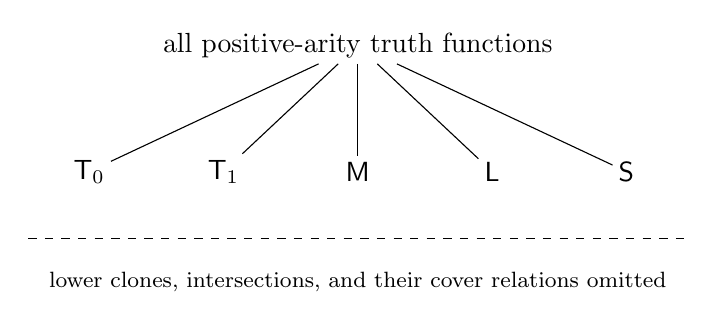
\begin{tikzpicture}[x=1.55cm,y=1cm,every node/.style={inner sep=2pt}]
 \node (all) at (2,3.8) {all positive-arity truth functions};
 \node (t0) at (-0.2,2.2) {\(\mathsf T_0\)};
 \node (t1) at (0.9,2.2) {\(\mathsf T_1\)};
 \node (m)  at (2.0,2.2) {\(\mathsf M\)};
 \node (l)  at (3.1,2.2) {\(\mathsf L\)};
 \node (s)  at (4.2,2.2) {\(\mathsf S\)};
 \draw (all)--(t0); \draw (all)--(t1); \draw (all)--(m);
 \draw (all)--(l); \draw (all)--(s);
 \draw[dashed] (-0.7,1.35)--(4.7,1.35);
 \node[font=\footnotesize,align=center] at (2,0.8)
   {lower clones, intersections, and their cover relations omitted};
\end{tikzpicture}
\caption{Upper cover of Post's clone lattice: the five
displayed nodes are precisely the coatoms.  The dashed boundary deliberately
does not identify the extensive lower lattice with a single node
(apparatus A-119).}
\label{fig:p02-post-lattice}
\end{figure}
